\documentclass{suturo}

\begin{document}
    \maketitle{Planning}{02.01.2017}{}{1}{}{}{}{}

\makeatletter
\newcommand{\chapterauthor}[1]{%
  {\parindent0pt\vspace*{-27pt}%
  \linespread{0}\small\begin{flushright}von: #1\end{flushright}%
  \par\nobreak\vspace*{0pt}}
  \@afterheading%
}
\makeatother

\section{Node: main (planning\_main\_programm)}
\subsection{Architekturbild}
\chapterauthor{Kevin Störmer}
\begin{center} 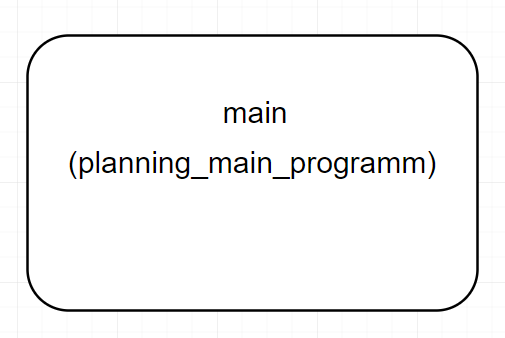
\includegraphics[width=0.4\textwidth]{img/diag_planning_main_programm.png} \end{center}
\subsection{Beschreibung des Teilsystems}
\subsubsection{\"Ubersicht}
\chapterauthor{Kevin Störmer}
Die Node 'main' im Paket 'planning\_main\_programm' soll ausschliesslich auf höchster Ebene den internen Ablauf des PR2 modellieren. Dabei wird der folgende Ablauf sequenziell ausgef\"uhrt:\\
(TOLLES SCHAUBILD)\\ \\
Alle dafür notwendigen Logiken, die auf Basis externer Daten entschieden werden, wurden dabei basierend auf der Quelle der Daten in andere Nodes ausgelagert. Dabei wurde z.b der Vergleich zweier Punkte aus Vision in die Node 'points' (Paket: planning\_vision) ausgelagert.

\section{Node: points (planning\_vision)}
\subsection{Architekturbild}
\chapterauthor{Kevin Störmer}
\begin{center} 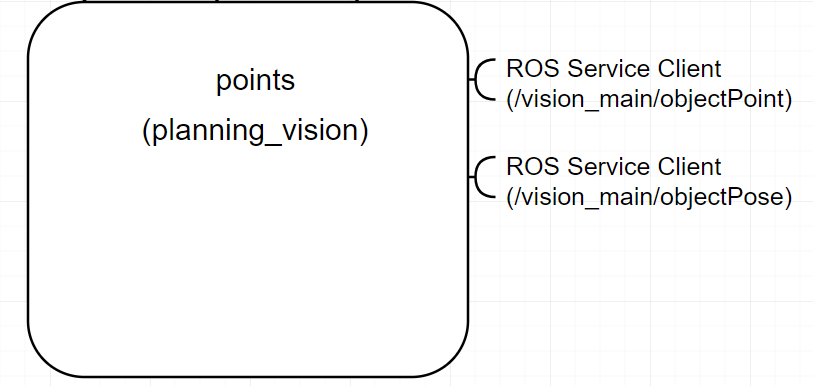
\includegraphics[width=0.6\textwidth]{img/diag_planning_vision.png} \end{center}
\subsection{API}
\chapterauthor{Kevin Störmer}
\subsubsection{Serviceclients}
1. '/vision\_main/objectPoint' \\
Nimmt Objekt über Kinect wahr, und gibt Mittelpunkt des Objektes zur\"uck.\\ \\
2. '/vision\_main/objectPose' \\
Nimmt Pose (steht oder liegt) des Objektes wahr.
\subsection{Beschreibung des Teilsystems}
\subsubsection{\"Ubersicht}
\chapterauthor{Kevin Störmer}
Die Node 'points' aus dem Paket 'planning\_vision' befasst sich ausschliesslich mit der Kommunikation mit Gruppe-Vision und Logiken auf Basis der wahrgenommenen Daten. Dabei werden Services zur Position und Pose des Objectes in Anspruch genommen und ausgewerten. Zudem wird eine Methode zur Validierung zweier Punkte angeboten.

\subsubsection{check-points-is-equal (msg-one msg-two delta)}
\chapterauthor{Kevin Störmer}
\begin{lstlisting}
(defun check-points-is-equal (msg-one msg-two delta)
  "Compares two points with delta."
  (roslisp::ros-info "check-points-is-equal" "Starting to check if point of object is still valid")
  (roslisp:with-fields ((x1 (geometry_msgs-msg:x geometry_msgs-msg:point)) 
                        (y1 (geometry_msgs-msg:y geometry_msgs-msg:point))
                        (z1 (geometry_msgs-msg:z geometry_msgs-msg:point)))
     (object_detection-msg:position (object_detection-srv:object msg-one))
     (roslisp:with-fields ((x2 (geometry_msgs-msg:x geometry_msgs-msg:point)) 
                           (y2 (geometry_msgs-msg:y geometry_msgs-msg:point))
                           (z2 (geometry_msgs-msg:z geometry_msgs-msg:point)))
                        (object_detection-msg:position (object_detection-srv:object msg-two))
       (let (
             (dx (abs (- x1 x2)))
             (dy (abs (- y1 y2)))
             (dz (abs (- z1 z2)))
             )
         (if (and
              (<= dx delta)
              (<= dy delta)
              (<= dz delta)
              )
             (print t)
             (print nil)
             )
         )
       )
    )
  )
\end{lstlisting}

Die Funktion 'check-points-is-equal' bekommt die Parameter 'msg-one' und 'msg-two' \"ubergeben. Dabei handelt es sich um Messages vom Typ 'object\_detection-msg'. Diese enthalten Punke (x, y, z) die zu verschiedenen Zeiten von Vision über die Kinect wahrgenommen wurden. Sie stellen den Mittelpunkt des umzustossenden Objektes dar. Beim \"Ubergabeparameter delta, handelt es sich um die maximale erlaubte Tolleranz mit der die beiden Punkte von einander abweichen dürfen. \\
Anf\"anglich werden die Koordinaten der beiden Messages aus den Wrappern extrahiert und in Variablen fortan verf\"ugbar gemacht. Danach werden die Koordinaten paarweise voneinander subtrahiert um die Differenz beider als vorzeichenlose Zahl zu errechnen. Diese Differenz wird dann mit dem vorgegebenen Delta verglichen. Wenn sich alle Differenzen innerhalb des Deltas befinden, wird 'true' zurückgegeben, sonst 'nil'. 

\subsubsection{call-vision-point ()}
\chapterauthor{Hauke Tietjen}
\begin{lstlisting}
(defvar not-a-number)

(defun call-vision-point ()
  "Call vision service, to look for point. Returns ObjectDetection object"
  (cpl:with-retry-counters ((retry-counter 10))
    (cpl:with-failure-handling
        ((cpl:simple-plan-failure (error-object)
           (format t "An error happened: ~a~%" error-object)
           (cpl:do-retry retry-counter
             (format t "Now retrying~%")
             (cpl:retry))
           (format t "Reached maximum amount of retries. Now propagating the failure up.~%")))
      (let ((response
              (roslisp:call-service
               "/vision_main/objectPoint"
               'object_detection-srv:visobjectinfo)))
        ;;Debug to find NaN message from vision
        (setf not-a-number response)
        (print not-a-number)
        (roslisp:with-fields ((x (geometry_msgs-msg:x geometry_msgs-msg:point)) 
                              (y (geometry_msgs-msg:y geometry_msgs-msg:point))
                              (z (geometry_msgs-msg:z geometry_msgs-msg:point)))
            (object_detection-msg:position (object_detection-srv:object response))
          ;;If Vision returns a NaN and it is of type String this will recover from the error
          (if (or (stringp x)
                  (stringp y)
                  (stringp z))
              (cpl:fail "One or more of the coordinates returned by the service /vision_main/objectPoint is of type String
                        which is likely the not a number error")
              (if (or (sb-ext:float-nan-p x)
                      (sb-ext:float-nan-p y)
                      (sb-ext:float-nan-p z))
                  (cpl:fail "One or more of the coordinates returned by the service /vision_main/objectPoint is  not a number")
                  (roslisp:with-fields (object_detection-msg:error) (object_detection-srv:object response)
                    (if (or (string= "Cloud empty. " object_detection-msg:error)
                            (string= "Cloud was empty after filtering. " object_detection-msg:error)
                            (string= "No plane found. " object_detection-msg:error)
                            (string= "Final extracted cluster was empty. " object_detection-msg:error))
                        (cpl:fail (concatenate 'string "Service call failed: " object_detection-msg:error))
                        (progn
                          (format t "Service call successful.")
                          (return-from call-vision-point
                            (roslisp:call-service "/vision_main/objectPoint" 'object_detection-srv:VisObjectInfo))))))))))))
\end{lstlisting}

Die Funktion 'call-vision-point' ruft den Service '/vision\_main/objectPoint' von Vision auf. Dieser Service gibt den Mittelpunkt des gesehenen Objekts zurück welcher dann nach einer Fehlerüberpüfung als 'object\_detection-msg' zurückgegeben wird. 

In Gazebo gibt dieser Service manchmal ein 'not a number' zurück, daher wird der Rückgabewert daraufhin überprüft. Es ist noch nicht klar ob 'NaN' als String oder float übergeben wird, daher wird beides überprüft. Zu 'sb-ext:float-nan-p' muss man sagen das es überprüft ob die nachfolgende Variable ein 'NaN' enthält und falls ja 't' zurückgibt, weil dazu keine Dokumentation auffindbar ist. Dann werden noch die bereitgestellten Fehlermeldungen von Vision abgefragt, z.B. ob überhaupt ein Objekt gesehen wurde. Falls mindestens eine dieser Abfragen zutrifft wird der Service-Call und die Fehlerüberprüfung neu gestartet. Dadurch kann die Funktion bis zu zehn mal neu gestartet werden bis sie endgültig aufgibt. Hier könnte in Zukunft eine Funktion auf höherem Level anknüpfen und den Kopf oder den ganzen Roboter bewegen um das Objekt doch noch zu erkennen.

\section{Node: ask (planning\_knowledge)}
\subsection{Architekturbild}
\chapterauthor{Kevin Störmer}
\begin{center} 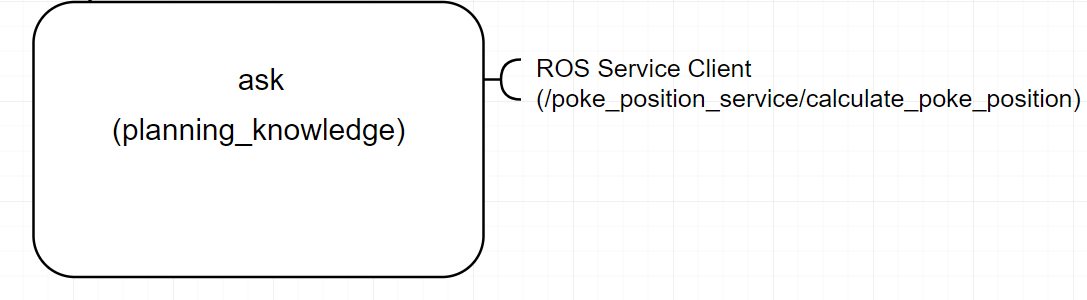
\includegraphics[width=0.8\textwidth]{img/diag_planning_knowledge.png} \end{center}
\subsection{API}
\chapterauthor{Kevin Störmer}
\subsubsection{Serviceclients}
1. '/poke\_position\_service/calculation\_poke\_position' \\
Berechnet den zu stupsenden Punkt des Objektes
\subsection{Beschreibung des Teilsystems}
\subsubsection{\"Ubersicht}
\chapterauthor{Kevin Störmer}
Die Node 'ask' im Paket 'planning\_knowledge' ist ausschliesslich für die Kommunikation mit Gruppe Knowledge zust\"andig.
\subsubsection{ask-knowledge(point-center-of-object)}
\chapterauthor{Kevin Störmer}
Die Funktion 'ask-knowledge' bekommt als \"Ubergabeparameter eine 'object\_detection-msg' welche den, von Vision, wahrgenommenen Mittelpunkt des Objektes enthält. Knowledge gibt nach Aufruf des Services dann einen Punkt oberhalb des Mittelpunktes zur\"uck, welchen wir dann fortw\"ahrend in unserer Main weiterverwenden.

\section{Node: actions (planning\_motion)}
\subsection{Architekturbild}
\chapterauthor{Kevin Störmer}
\begin{center} 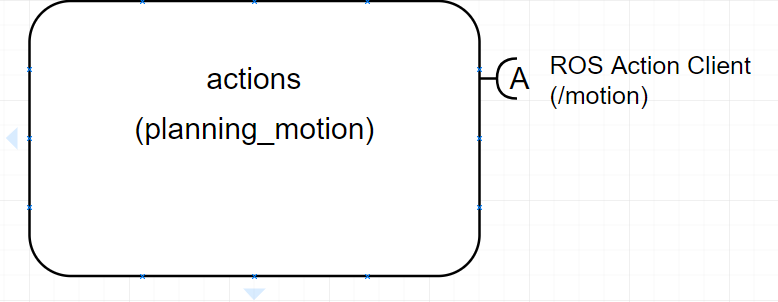
\includegraphics[width=0.6\textwidth]{img/diag_planning_motion.png} \end{center}
\subsection{API}
\chapterauthor{Kevin Störmer}
\subsubsection{Actionclients}
1. '/motion' \\
Bewegt die Arme des Pr2 entweder in die Home-Position oder zu einem bestimmten Punkt.
\subsection{Beschreibung des Teilsystems}
\subsubsection{\"Ubersicht}
\chapterauthor{Kevin Störmer}
Die Node 'actions' im Paket 'planning\_motion'  ist ausschliesslich für die Kommunikation mit Gruppe Motion zuständig. Dabei wird die Action '/motion' einmal für die Home-Position des Pr2 und zum Bewegen des Armes zu einem bestimmten Punkt genutzt.

\section{Node: movement (planning\_move)}
\subsection{Architekturbild}
\chapterauthor{Kevin Störmer}
\begin{center} 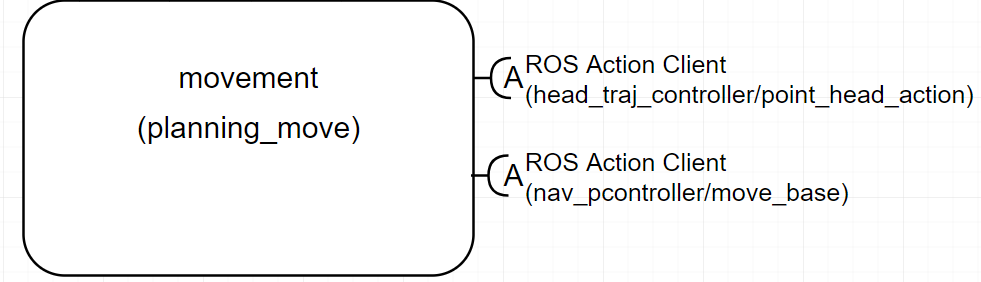
\includegraphics[width=0.8\textwidth]{img/diag_planning_move.png} \end{center}
\subsection{API}
\chapterauthor{Kevin Störmer}
\subsubsection{Actionclients}
1. 'head\_traj\_controller/point\_head\_action' \\
Bewegt den Kopf des Pr2 in Richtung eines Punktes.\\ \\
2. 'nav\_pcontroller/move\_base' \\
Bewegt die Basis des Pr2 in Richtung eines Punktes.
\subsection{Beschreibung des Teilsystems}
\subsubsection{\"Ubersicht}
\chapterauthor{Kevin Störmer}
Die Node 'movement' im Paket 'planning\_move' behandelt alle Fälle in denen sich der Pr2 bewegen soll, welche nicht von Gruppe Motion abgehandelt werden. Dabei eine Methode zum Bewegen des Kopfes des Pr2 angeboten sowie eine Methode zum Bewegen der Basis des Pr2.
\subsubsection{move-head (x y z)}
\chapterauthor{Kevin Störmer}
\begin{lstlisting}
(defun move-head (x y z)
   "Moving robot head via head_traj_controller/point_head_action. X Y Z are treated as coordinates."
     (let ((actionclient 
            (actionlib:make-action-client "head_traj_controller/point_head_action" "pr2_controllers_msgs/PointHeadAction")))
       (loop until
            (actionlib:wait-for-server actionclient))
       (let ((point-to-look-at 
            (cl-transforms-stamped:to-msg 
            (cl-transforms-stamped:make-point-stamped "base_link" 0 
                                                       (cl-transforms:make-3d-vector x y z)))))
           (let ((actiongoal 
               (actionlib:make-action-goal actionclient target point-to-look-at)))
               (actionlib:call-goal actionclient actiongoal)))))
\end{lstlisting}
Die Funktion 'move-head' bekommt als \"Ubergabeparameter Koordinaten (x y z) welche vorgeben sollen, in welche Richtung der Kopf des Pr2 bewegt wird.\\
Zuerst wird ein neuer Actionclient, für die 'head\_traj\_controller/point\_head\_action' Action erstellt. Anschliessend soll in einem Loop solange gewartet werden, bis der Actionsserver gestartet wurde. Ist dies der Fall, wird eine neue Message erstellt, welche einen Punkt auf Basis der \"ubergebenen Koordinaten, in Relation zum Frame 'base\_link', enth\"alt. Diese wird dann in ein neues Actiongoal gefasst und an den Actionserver geschickt, welcher den Kopf des Pr2 dann in Richtung der Koordinaten bewegen wird.


\subsubsection{move-Base-To-Point (x y z w)}
\chapterauthor{Kevin Störmer}
\begin{lstlisting}
(defun move-Base-To-Point (x y z w)
  "Moving robot base via nav_pcontroller/move_base. X Y Z are treated as coordinates. W for Orientation."
  (let ((actionclient 
         (actionlib:make-action-client "nav_pcontroller/move_base" "move_base_msgs/MoveBaseAction")))
     (loop until
             (actionlib:wait-for-server actionclient))
     (let ((pose-to-drive-to 
            (cl-transforms-stamped:to-msg 
            (cl-transforms-stamped:make-pose-stamped "base_link" 0 
                                                 (cl-transforms:make-3d-vector x y z) (cl-tf:make-quaternion x y z w)))))
         (let ((actiongoal 
                 (actionlib:make-action-goal actionclient target_pose pose-to-drive-to)))
                 (actionlib:call-goal actionclient actiongoal)))))
\end{lstlisting}
Die Funktion 'move-Base-To-Point' hat es nicht auf den Roboter geschafft, und ist momentan auch nicht korrekt. Sie konnte aus Zeitmangel nicht weiterentwickelt werden.\\
Angedacht war es, dass eine Pose anhand von Übergabeparametern erstellt wird, und über den Actionserver des Navp-controllers den Roboter in die vorgesehene Pose zu bewegen. Dabei traten allerdings Probleme auf, die wir zeitlich nicht mehr reparieren konnten.
\end{document}
